\begin{figure}[!htbp]
    \begin{subfigure}{.48\textwidth}
        \centering
        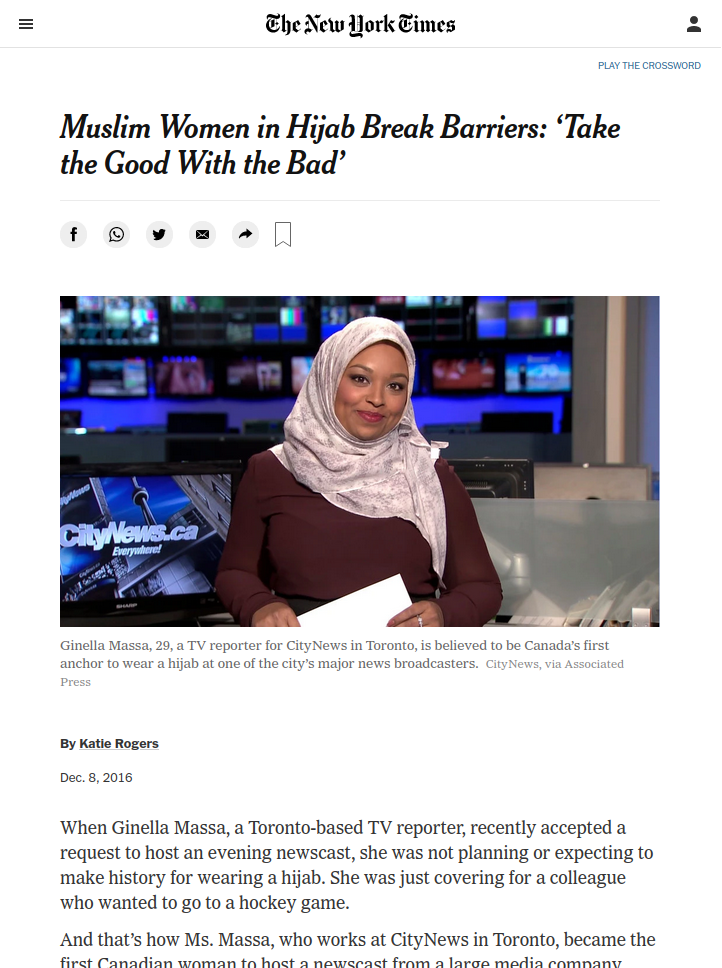
\includegraphics[scale=0.28]{4_kptimes/figures/image_kptimes.png}
        \caption{Capture d'écran d'un article sur le site du New York Times.}
        \label{fig:img_kptimes}
    \end{subfigure}%
    \hfill
    \begin{subfigure}{.48\textwidth}
\begin{minted}[
frame=lines,framesep=2mm,
baselinestretch=0.9,fontsize=\scriptsize
]{html}
<html><body>
<title>Muslim Women in Hijab Break Barriers:
‘Take the Good With the Bad’ - The New York
Times</title>
<meta name="description" content="
    Even as reports of hate crimes against 
    Muslims rise in America and Canada, 
    hijabis are appearing in makeup ads, 
    beauty pageants and news anchor chairs.
    ">
<meta name="byl" content="By Katie Rogers">
<meta name="news_keywords" content="
    Muslim Veiling,,Hate crime, Women and 
    Girls,Canada,US,Islam,Fashion,
    News media;journalism,">
<meta name="CG" content="world">
<meta name="SCG" content="americas">
<meta name="pdate" content="20161208">
<meta name="url" content="
    https://www.nytimes.com/2016/12/08/
    world/americas/hijab-muslim-women.html">
...
</head><body>
When Ginella Massa, a Toronto-based ...
</body></html>
\end{minted}
    \caption{Code source d'un article du site du New York Times.}
    \label{fig:meta_kptimes}
\end{subfigure}%
    
    
    \iffalse
    \begin{subfigure}{.48\textwidth}
        \centering
        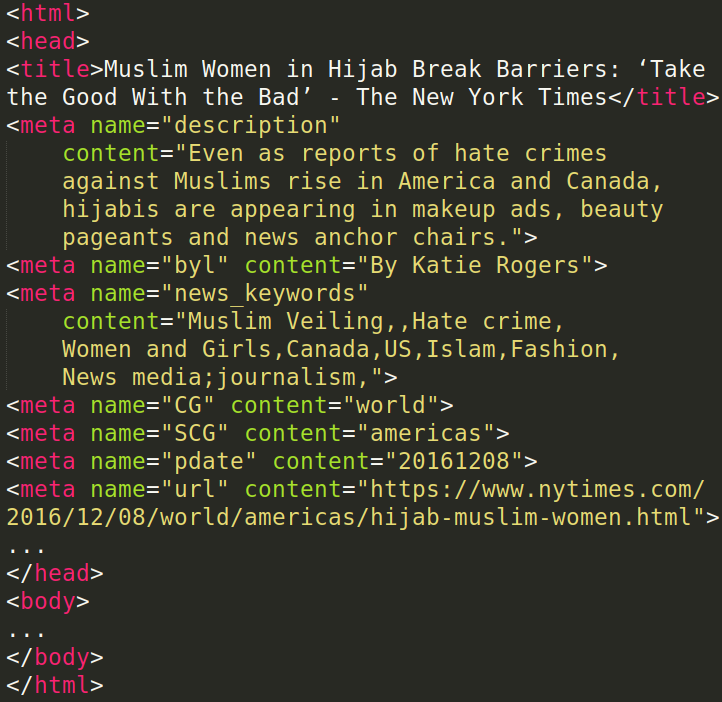
\includegraphics[scale=0.27]{4_kptimes/figures/html_kptimes.png}
        \caption{Code source d'un article du site du New York Times.}
        \label{fig:meta_kptimes}
    \end{subfigure}%
    \fi
    \caption{Version web et \texttt{html} de l'article \texttt{ny0296216} du jeu de données KPTimes.}
    \label{fig:kptimes_ex_img}
\end{figure}